\renewcommand{\chaptername}{\scshape Partie}
\chapter{\normalfont \scshape Dispositif à onde de choc}
\section{Théorie du tube à choc}
Une onde de choc est une onde créée par une transition brutale~\ref{ref:wiki_choc}, donc une discontinuité, de grandeurs physiques comme la pression, la masse volumique ou encore la vitesse.
Pour pouvoir obtenir une onde de choc, on utilise un tube à choc. Le tube à choc sert à  reproduire et concentrer des ondes de choc en simulant des explosions.
Ici, le tube à choc permet la création d’ondes grâce à la discontinuité en pression à l’intérieur de ce dernier.\\
\begin{figure}[H]
	\centering
	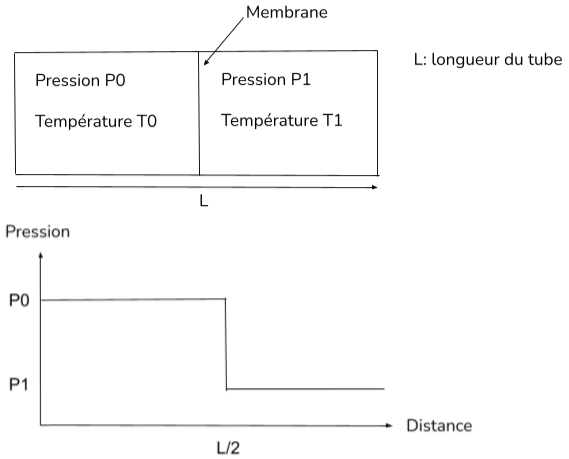
\includegraphics[scale = 0.4]{figures/principe_choc.png}
	\caption{\small{\textit{Principe et évolution de la pression dans le tube à choc}}}
	\label{fig:principe_choc}
\end{figure}
Le tube à choc est composé de deux tubes en PVC séparés par une membrane. En pompant la partie gauche du montage à l'aide de la pompe à vélo, on augmente la pression dans le tube de gauche. A partir d'une pression P, la membrane se brise et la discontinuité de pression dans le tube crée l'onde de choc et par conséquent l'explosion à la sortie du tube.\\
Le but de cette étape du projet est d'exploiter ce principe pour générer une onde de choc.
\section{Protocole et organisation}
\subsection{Cahier des charges}
Après avoir déterminé les objectifs techniques, le diagramme de GANTT suivant a été établi :
\begin{figure}[H]
	\centering
	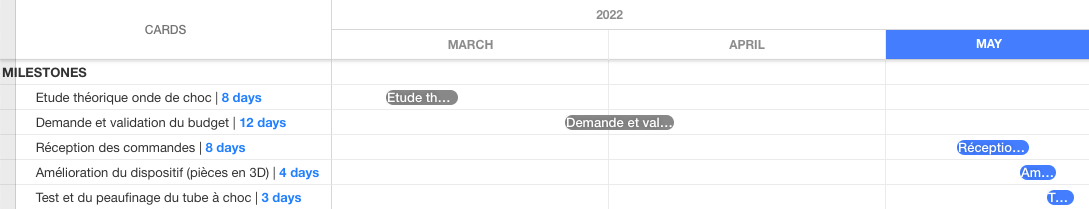
\includegraphics[scale = 0.4]{figures/gantt_choc.png}
	\caption{\small{\textit{Diagramme de GANTT prévu pour le dispositif à onde de choc}}}
	\label{fig:gantt_choc}
\end{figure}
Le travail sur le tube à onde de choc a été confié aux trois membres restants du groupe. Le tableau~\ref{tab:gestion_choc} résume les postes attribués à chacun des membres:
\begin{table}[H]
	\centering
	\begin{tabular}{|l l l|}
		\hline
		\small\textbf{Responsable onde de choc}&\small\textbf{Responsable budget}&\small\textbf{Responsable technique}\\
		\hline
		\small{Hovanes BOKSYAN}&\small{Nino VIVIAND}&\small{Aymeric FREREJEAN}\\
		\hline
	\end{tabular}
	\caption{\small\textit{Membres et tâches attribuées (tube à onde de choc)}}
	\label{tab:gestion_choc}
\end{table}
\subsection{Mise en place du dispositif}
\subsubsection{\normalfont{\textsc{$1^{er}$ essai : onde de choc hydraulique}}}
Dans un premier temps, un test a été effectué grâce à une pompe hydraulique après avoir rempli une cuve d’eau à entrée réglable. Avec l’entrée bloquée par une vanne, un flux d’eau a été envoyé puis bloqué par la vanne et à un instant t, la vanne a été débloquée et a permis l’observation d’une onde de choc hydraulique (cf. figure~\ref{fig:choc_hydro}).
\begin{figure}[H]
	\centering
	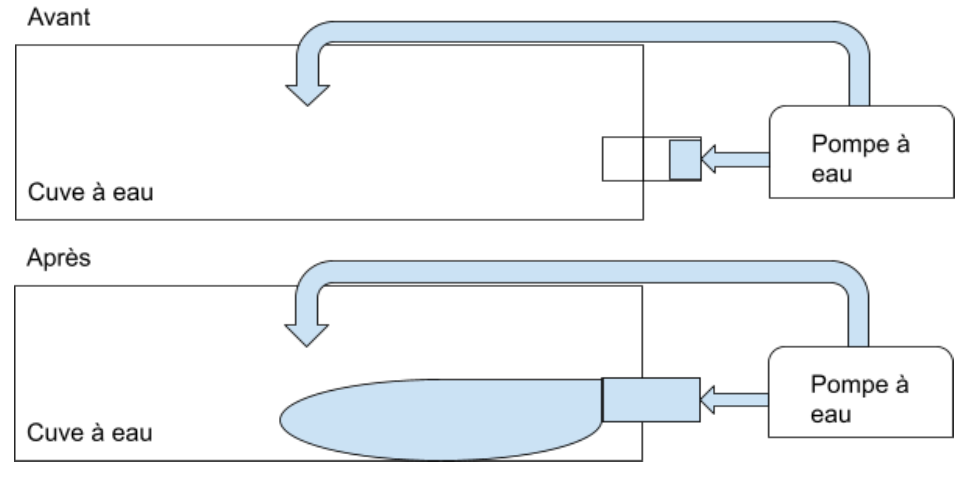
\includegraphics[scale = 0.4]{figures/choc_hydro.png}
	\caption{\small{\textit{Schéma du test réalisé à l'aide de la pompe hydraulique}}}
	\label{fig:choc_hydro}
\end{figure}
\subsubsection{\normalfont{\textsc{Test final de l'onde de choc}}}
Une fois le principe de l'onde de choc testé sur la pompe hydraulique, on procède aux tests avec pompe à air.
\begin{figure}[H]
	\centering
	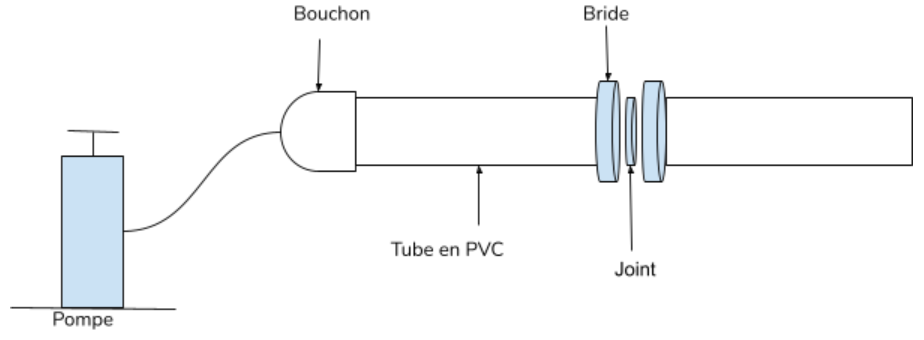
\includegraphics[scale = 0.4]{figures/choc_air.png}
	\caption{\small{\textit{Schéma du dispositif construit pour l'onde de choc finale}}}
	\label{fig:choc_air}
\end{figure}
Pour réaliser le tube à choc de la figure~\ref{fig:choc_air}, le matériel suivant a été utilisé~\ref{ref:zigunov}:
\begin{itemize}
	\item 1 tube en PVC : \textbf{ø 40 mm}, \textbf{$\mathnormal{L}$ = 1 m} (dimensions habituelles);
	\item 1 bouchon à coller en PVC : \textbf{ø 40 mm} pour éviter la fuite d'air d'un côté du tube;
	\item 1 colle PVC;
	\item 2 brides : \textbf{ø 40 mm};
	\item 4 vis et écrous;
	\item 1 pompe à pied;
	\item 1 joint en caoutchouc.
\end{itemize}
Le budget total du dispositif s'est élevé à \textbf{55,86 €}.
Entre le joint et la bride de droite est placée la membrane dont le matériau doit être déterminé. 
\section{Observations et conclusion}
\subsection{Observations}
Afin de choisir le matériau adéquat pour la membrane, une série de tests a été effectuée. En effet, le matériau utilisé sur le site web consulté~\ref{ref:zigunov} qui a inspiré la conception du dispositif était difficilement trouvable en France. Par conséquent, une étude des matériaux dont les caractéristiques se rapprochent d’une feuille PVC de 70 µm a été réalisée.\\
Le tableau~\ref{tab:choc_resultats} résume les résultats obtenus selon le matériau utilisé pour la membrane.\\
\begin{table}[H]
	\centering
	\begin{tabular}{|l|l|l|l|l|l|l|}
		\hline
		&\vtop{\hbox{\strut \small{Feuille de}}\hbox{\strut \small{plastifieuse}}\hbox{\strut \small{(e = 75 µm)}}}&\vtop{\hbox{\strut \small{Feuille}}\hbox{\strut \small{trans-}}\hbox{\strut \small{parente}}\hbox{\strut \small{(feuille de}}\hbox{\strut \small{classeur)}}}&\vtop{\hbox{\strut \small{Feuille de}}\hbox{\strut \small{papier}}\hbox{\strut \small{impri-}}\hbox{\strut \small{mante}}}&\vtop{\hbox{\strut \small{Mouchoirs}}\hbox{\strut \small{en papier}}}&\vtop{\hbox{\strut \small{Rouleau}}\hbox{\strut \small{adhésif}}\hbox{\strut \small{emballage}}\hbox{\strut \small{(ultra}}\hbox{\strut \small{résistant)}}}&\vtop{\hbox{\strut \bfseries\small{Rouleau}}\hbox{\strut \bfseries\small{adhésif}}\hbox{\strut \bfseries\small{type}}\hbox{\strut \bfseries\small\textit{Gaffer}}}\\
		\hline
		\vtop{\hbox{\strut \small{Pression}}\hbox{\strut \small{avant}}\hbox{\strut \small{rupture}}}&\vtop{\hbox{\strut \small{Pas de}}\hbox{\strut \small{rupture}}}&\vtop{\hbox{\strut \small{Pas de}}\hbox{\strut \small{rupture}}}&\vtop{\hbox{\strut \small{Pas de}}\hbox{\strut \small{rupture}}}&\small{< 1 bar}&\vtop{\hbox{\strut \small{Pas de}}\hbox{\strut \small{rupture}}}&\vtop{\hbox{\strut \small{\bfseries$\simeq$ 2,5}}\hbox{\strut \small{\small\bfseries bars}}}\\
		\hline
		\vtop{\hbox{\strut \small{Comm-}}\hbox{\strut \small{entaire}}}&\vtop{\hbox{\strut \small{Tests}}\hbox{\strut \small{jusqu'à 4}}\hbox{\strut \small{bars.}}\hbox{\strut \small{Fuites d'air}}\hbox{\strut \small{empêchant}}\hbox{\strut \small{l'augmentation}}\hbox{\strut \small{de la pression}}\hbox{\strut \small{(la feuille}}\hbox{\strut \small{se tord}}\hbox{\strut \small{sous la}}\hbox{\strut \small{contrainte).}}\hbox{\strut \small{Déformation}}\hbox{\strut \small{plastique}}\hbox{\strut \small{à partir}}\hbox{\strut \small{de 4 bars.}}}&\vtop{\hbox{\strut \small{Tests}}\hbox{\strut \small{jusqu'à 3}}\hbox{\strut \small{bars.}}\hbox{\strut \small{Trop de}}\hbox{\strut \small{déform-}}\hbox{\strut \small{ation}}\hbox{\strut \small{avant}}\hbox{\strut \small{rupture.}}\hbox{\strut \small{Matériau}}\hbox{\strut \small{trop}}\hbox{\strut \small{élastique.}}}&\vtop{\hbox{\strut \small{Tests}}\hbox{\strut \small{jusqu'à 3}}\hbox{\strut \small{bars.}}\hbox{\strut \small{Trop de}}\hbox{\strut \small{fuites d'air}}\hbox{\strut \small{car la}}\hbox{\strut \small{feuille}}\hbox{\strut \small{se tord}}\hbox{\strut \small{sous la}}\hbox{\strut \small{pression.}}}&\vtop{\hbox{\strut \small{Tests}}\hbox{\strut \small{réalisés}}\hbox{\strut \small{avec 1 à 8}}\hbox{\strut \small{couches.}}\hbox{\strut \small{Rupture}}\hbox{\strut \small{à trop}}\hbox{\strut \small{basse}}\hbox{\strut \small{pression}}\hbox{\strut \small{pour créer}}\hbox{\strut \small{une onde}}\hbox{\strut \small{de choc.}}}&\vtop{\hbox{\strut \small{Tests}}\hbox{\strut \small{jusqu'à 5}}\hbox{\strut \small{bars.}}\hbox{\strut \small{Pas de}}\hbox{\strut \small{rupture}}\hbox{\strut \small{avec une}}\hbox{\strut \small{seule}}\hbox{\strut \small{couche.}}\hbox{\strut \small{Imposs-}}\hbox{\strut \small{ible}}\hbox{\strut \small{d'augm-}}\hbox{\strut \small{enter la}}\hbox{\strut \small{pression}}\hbox{\strut \small{car trop}}\hbox{\strut \small{risqué.}}\hbox{\strut \small{Matériau}}\hbox{\strut \small{trop}}\hbox{\strut \small{résistant.}}}&\bfseries\vtop{\hbox{\strut \small{Tests}}\hbox{\strut \small{réalisés}}\hbox{\strut \small{avec}}\hbox{\strut \small{une seule}}\hbox{\strut \small{couche.}}\hbox{\strut \small{Pas de}}\hbox{\strut \small{fuite}}\hbox{\strut \small{et une}}\hbox{\strut \small{défrom-}}\hbox{\strut \small{ation du}}\hbox{\strut \small{matériau}}\hbox{\strut \small{quasi-}}\hbox{\strut \small{ment pas }}\hbox{\strut \small{visible,}}\hbox{\strut \small{donc la}}\hbox{\strut \small{rupture}}\hbox{\strut \small{est nette.}}}\\
		\hline
	\end{tabular}
	\caption{\small\textit{Résultats obtenus en fonction du matériau utilisé pour la membrane}}
	\label{tab:choc_resultats}
\end{table}
Le matériau le plus concluant s’est avéré être le scotch type \textit{Gaffer}, il a donc été conservé pour réaliser un test filmé. Les images de la figure~\ref{fig:choc_filmee} ont été prises après avoir placé le canon du générateur à onde de choc en face d’un récipient rempli d’eau (1 seule couche de scotch, rupture à 2,5 bars) :\\
\begin{figure}[H]
	\centering
	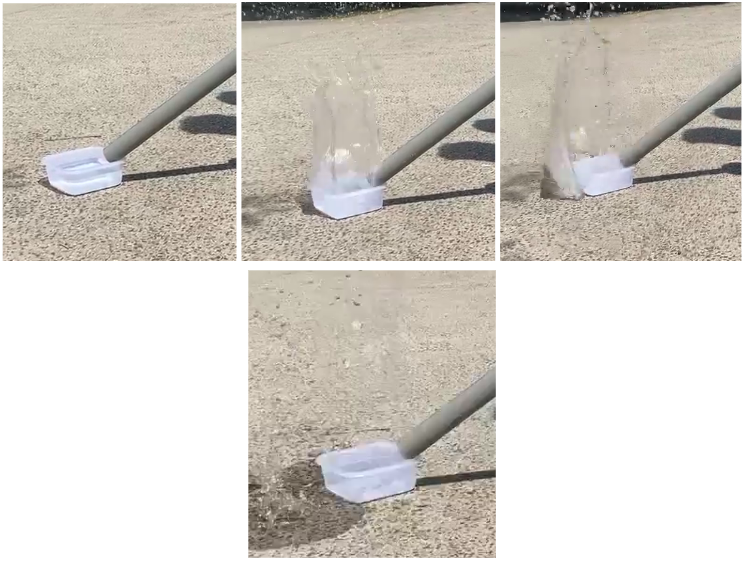
\includegraphics[scale = 0.5]{figures/choc_filmee.png}
	\caption{\small{\textit{Images de l'onde de choc générée, pression avant rupture : 2,5 bars}}}
	\label{fig:choc_filmee}
\end{figure}
On constate que, même à une pression de 2,5 bars, le système génère une résultat souhaité. En effet, trois éléments témoignent du passage de l’onde de choc : tout d'abord, on observe de fortes éclaboussures, ce qui montre bien la vitesse élevée de sortie de l'air. Les mouvements des gouttes d'eau sont accompagnés par un bruit sourd et de la fumée sortant du tuyau,comme le montre la dernière image de la figure~\ref{fig:choc_filmee}.\\\\
La figure~\ref{fig:choc_5bars} représente les images obtenues pour 2 couches de scotch, c'est-à-dire pour une pression avant rupture de 5 bars.\\
\begin{figure}[H]
	\centering
	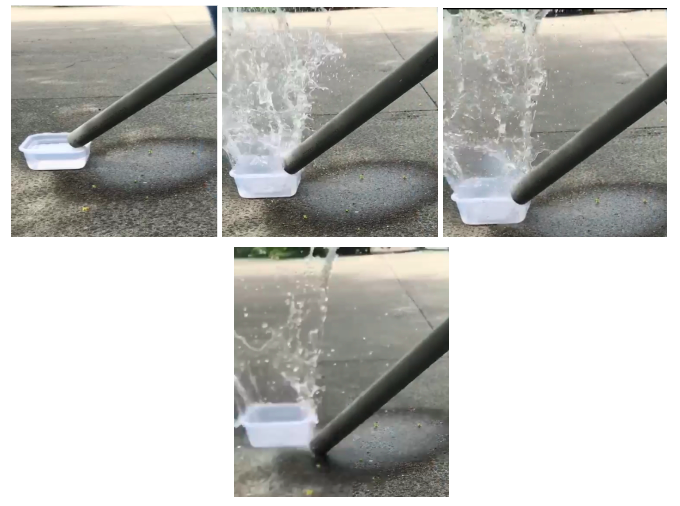
\includegraphics[scale = 0.5]{figures/choc_5bars.png}
	\caption{\small{\textit{Images de l'onde de choc générée, pression avant rupture : 5 bars}}}
	\label{fig:choc_5bars}
\end{figure}
En empilant plusieurs couches de scotch, il est possible d’augmenter la pression avant rupture selon une relation vraisemblablement linéaire (1 couche = 2,5 bars, 2 couches = 5 bars, etc..) et ainsi obtenir une onde de choc plus rapide. Cependant, une vitesse plus importante signifie une photographie à travers le dispositif Schlieren plus difficile à prendre. De plus, il faut prendre en compte l'aspect sécurité. Les pièces PVC sont censées résister à près de 10 bars, mais afin de limiter au maximum les risques d'explosion, on se limitera à 5,5 bars lors des tests. Une légère déformation des pièces imprimées en 3D a aussi été constatée lors des tests à deux couches de scotch. Enfin, le bruit est encore plus sourd et nécessite le port d'un casque antibruit. Pour toutes ces raisons, il a été décidé de se limiter à une seule couche de scotch \textit{Gaffer} pour les tests avec le dispositif optique.
\subsection{Conclusion partielle}
Les résultats obtenus montrent que le matériel choisi a permis d'obtenir une onde de choc. Cependant, la problématique demeure dans la capacité à obtenir une imagerie visible de l'onde avec le dispositif d'imagerie Schlieren, tout en tenant compte de la rapidité de la perturbation et des limites de l'appareil photo.